\section{实验二 时域采样与频域采样}

\subsection{一、实验流程图}
\begin{figure}[H]
\centering
\begin{tikzpicture}[
    node distance=1.8cm,
    auto,
    box/.style={rectangle, draw, text width=8.5em, align=center, minimum height=2.8em}
]
\node [box] (start) {开始};
\node [box, below of=start] (para) {设置参数\\信号、采样频率};
\node [box, below of=para] (time) {生成时域采样信号\\x(n)};
\node [box, below of=time] (fft) {FFT 求频谱};
\node [box, below of=fft] (plot1) {绘制时域波形\\+ 频谱};
\node [box, below of=plot1] (tri) {生成三角波序列};
\node [box, below of=tri] (fft2) {N=16 / 32 频域采样\\IFFT 还原};
\node [box, below of=fft2] (plot2) {绘制对比波形};
\node [box, below of=plot2] (end) {结束};

\draw [->] (start) -- (para);
\draw [->] (para) -- (time);
\draw [->] (time) -- (fft);
\draw [->] (fft) -- (plot1);
\draw [->] (plot1) -- (tri);
\draw [->] (tri) -- (fft2);
\draw [->] (fft2) -- (plot2);
\draw [->] (plot2) -- (end);
\end{tikzpicture}
\caption{实验二 采样与频谱分析流程图}
\end{figure}

\subsection{二、实验结果图像}
\begin{figure}[H]
    \centering
    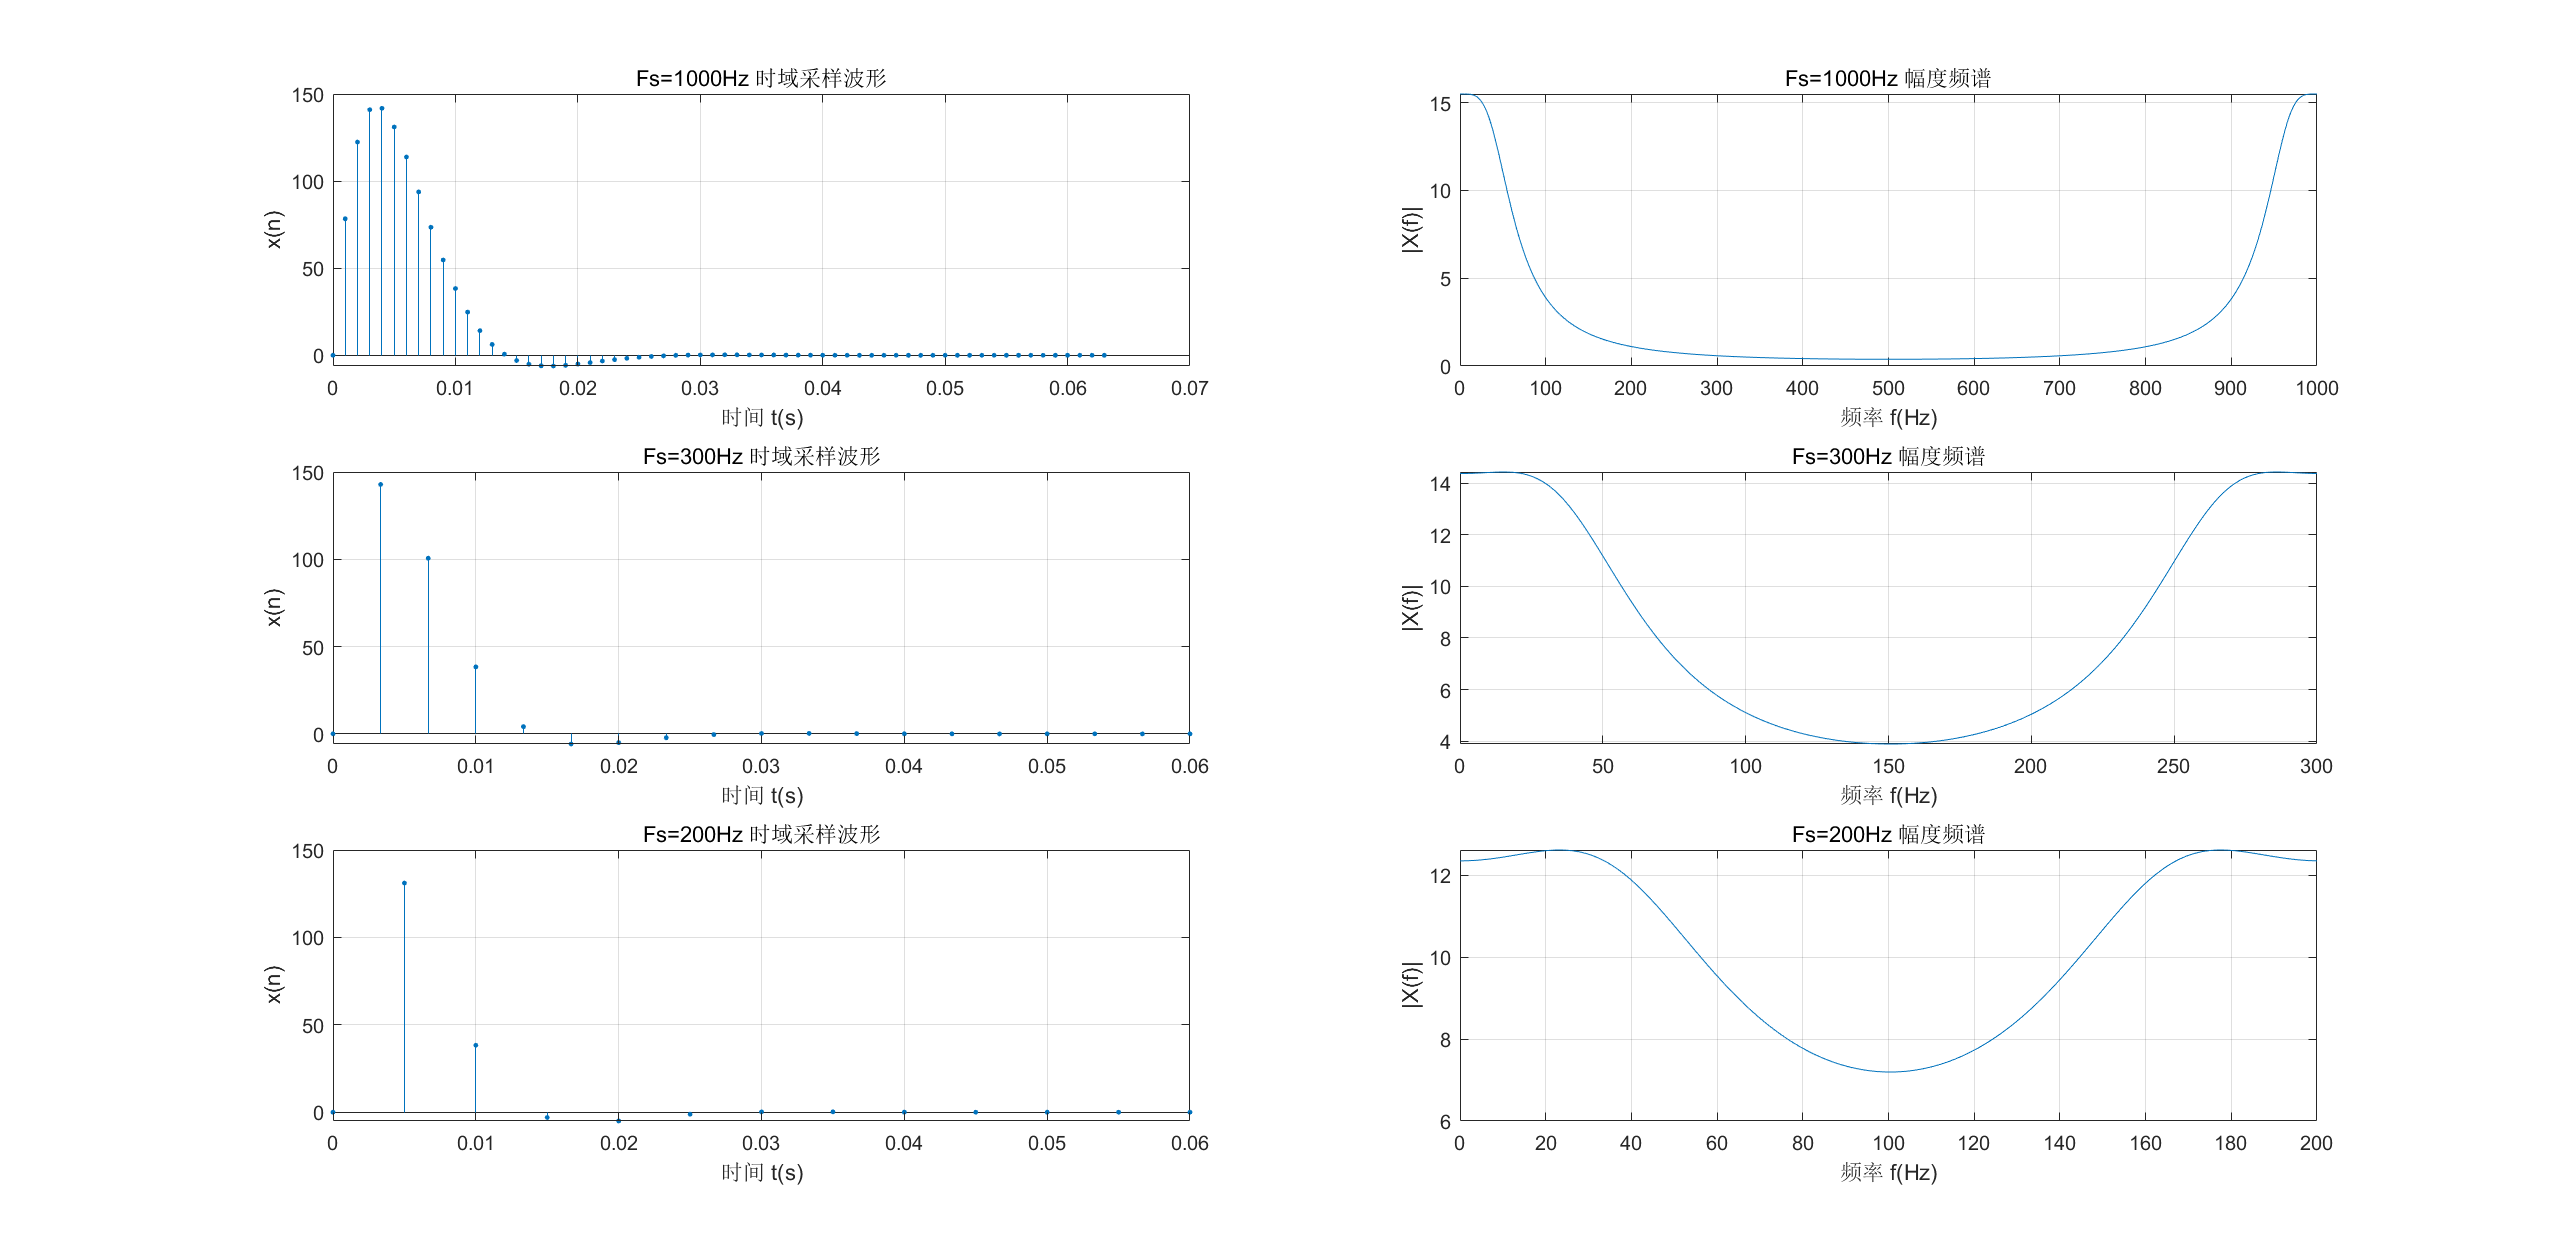
\includegraphics[width=0.85\textwidth]{2.1.png}
    \caption{时域采样波形与频谱图}
\end{figure}

\begin{figure}[H]
    \centering
    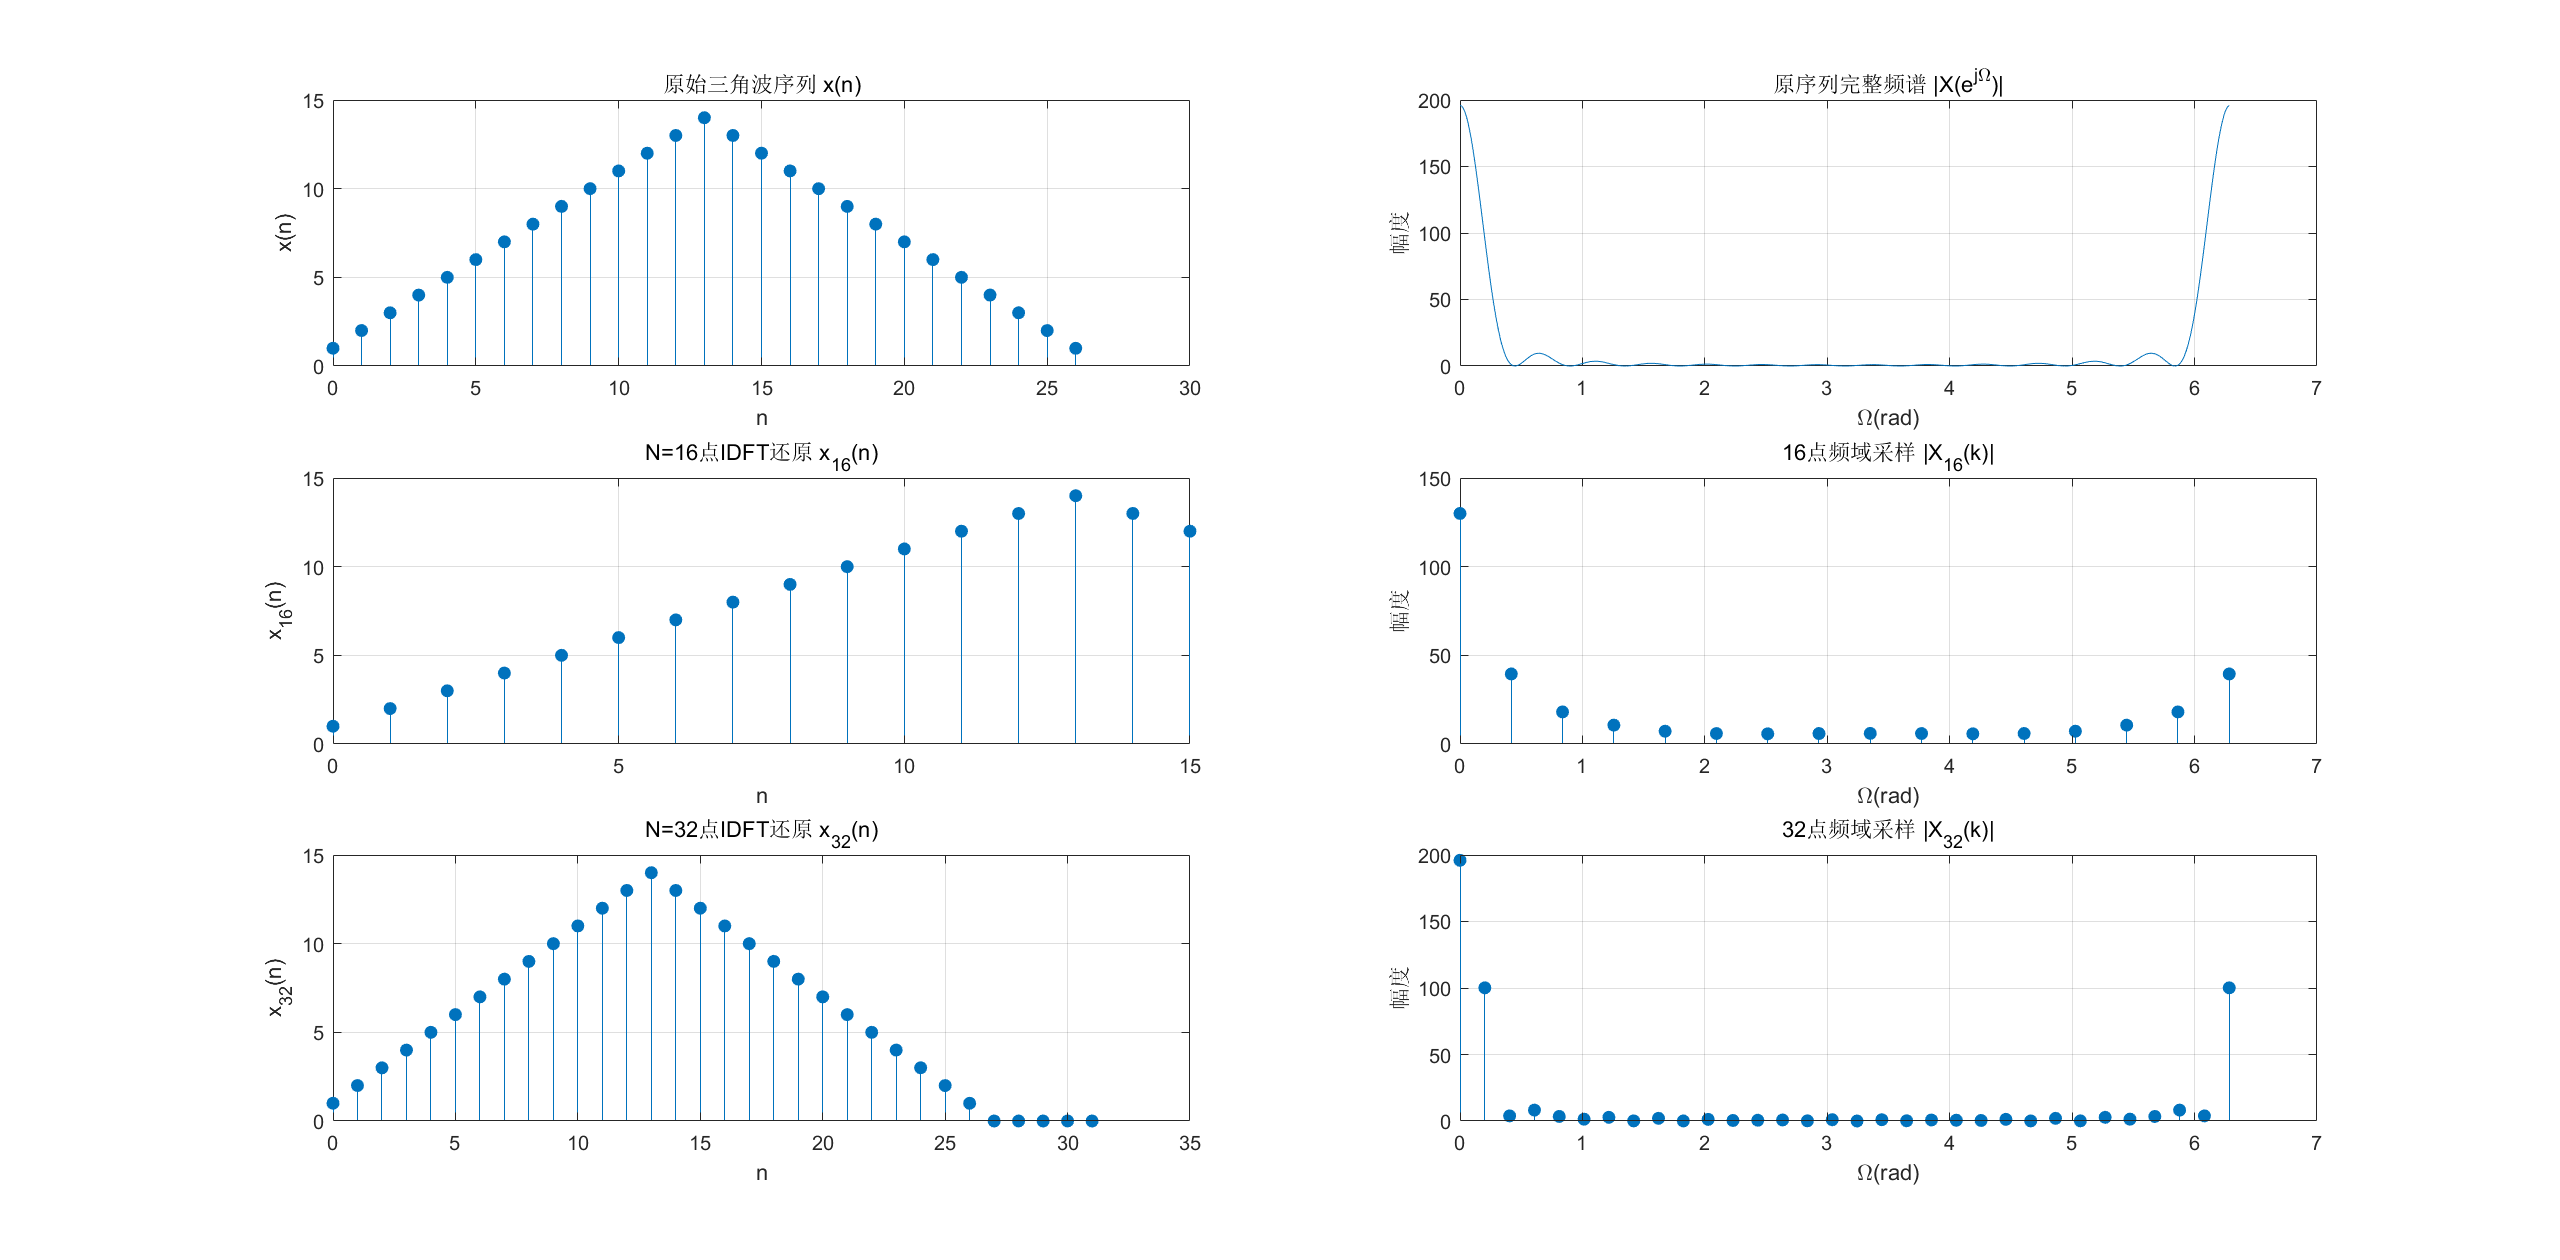
\includegraphics[width=0.85\textwidth]{2.2.png}
    \caption{频域采样与IDFT还原波形对比}
\end{figure}

\subsection{三、MATLAB 完整代码}
\subsubsection{1. 时域采样验证}
\begin{lstlisting}
clear; clc; close all;

A = 444.128;
alpha = 50*sqrt(2)*pi;
omega1 = 50*sqrt(2)*pi;
Tp = 0.064;
Fs_set = [1000,300,200];

figure('Name','时域采样验证');
for i = 1:3
    Fs = Fs_set(i);
    Ts = 1/Fs;
    N = round(Tp*Fs);
    n = 0:N-1;
    t = n*Ts;
    
    x = A.*exp(-alpha.*t).*sin(omega1.*t);
    
    NFFT = 2^nextpow2(N*10);
    Xk = fft(x,NFFT)/N;
    Amp = abs(Xk);
    f = linspace(0,Fs,NFFT);
    
    subplot(3,2,2*i-1);
    stem(t,x,'filled','MarkerSize',2);
    xlabel('时间 t(s)');ylabel('x(n)');
    title(['Fs=',num2str(Fs),'Hz 时域采样波形']);
    grid on;
    
    subplot(3,2,2*i);
    plot(f,Amp);
    xlabel('频率 f(Hz)');ylabel('|X(f)|');
    title(['Fs=',num2str(Fs),'Hz 幅度频谱']);
    thr = max(Amp)*0.005;
    idx = find(Amp>thr);
    if ~isempty(idx)
        xlim([f(idx(1)), f(idx(end))]);
    end
    grid on;
end
\end{lstlisting}

\subsubsection{2. 频域采样验证}
\begin{lstlisting}
clear; clc; close all;

M = 27;
n_x = 0:M-1;
x = zeros(1,M);
for nn = 0:M-1
    if nn <= 13
        x(nn+1) = nn+1;
    else
        x(nn+1) = 27-nn;
    end
end

N_full = 1024;
X_full = fft(x, N_full);
Amp_full = abs(X_full);
Om = linspace(0, 2*pi, N_full);

N32 = 32;
X32 = fft(x, N32);
x32 = real(ifft(X32, N32));

N16 = 16;
X16 = fft(x, N16);
x16 = real(ifft(X16, N16));

subplot(3,2,1);
stem(n_x, x, 'filled');
title('原始三角波序列 x(n)');
xlabel('n'); ylabel('x(n)'); grid on;

subplot(3,2,2);
plot(Om, Amp_full);
title('原序列完整频谱 |X(e^{j\Omega})|');
xlabel('\Omega(rad)'); ylabel('幅度'); grid on;

subplot(3,2,3);
stem(0:N16-1, x16, 'filled');
title('N=16点IDFT还原 x_{16}(n)');
xlabel('n'); ylabel('x_{16}(n)'); grid on;

subplot(3,2,4);
stem(linspace(0,2*pi,N16), abs(X16), 'filled');
title('16点频域采样 |X_{16}(k)|');
xlabel('\Omega(rad)'); ylabel('幅度'); grid on;

subplot(3,2,5);
stem(0:N32-1, x32, 'filled');
title('N=32点IDFT还原 x_{32}(n)');
xlabel('n'); ylabel('x_{32}(n)'); grid on;

subplot(3,2,6);
stem(linspace(0,2*pi,N32), abs(X32), 'filled');
title('32点频域采样 |X_{32}(k)|');
xlabel('\Omega(rad)'); ylabel('幅度'); grid on;
\end{lstlisting}

\subsection{四、实验思考题}
\begin{enumerate}
    \item 若序列长度为$M$，频域采样点数为$N$且$N<M$，如何用最少点数的DFT得到频域采样？
    
    \textbf{答：} 直接对原序列做 $N$ 点FFT即可，即 $X_N(k) = FFT(x(n),N)$，该操作等价于对频域进行 $N$ 点均匀采样，是最少点数的DFT实现方式。
    
    \item 时域采样实验中，为何可以用DFT（FFT）近似求解模拟信号的幅频特性？
    
    \textbf{答：} 模拟信号频谱是连续的，计算机无法直接计算；DFT是对连续频谱的等间隔采样，FFT是DFT的快速算法，因此可以用FFT近似表示模拟信号的幅频特性。
\end{enumerate}